\documentclass[border=6pt]{standalone}
\usepackage{tikz}
\usepackage{helvet}
\renewcommand{\familydefault}{\sfdefault}
\usetikzlibrary{arrows.meta, positioning, calc, backgrounds}

\definecolor{exprblue}{RGB}{70,130,180}   % steelblue, matches ledger x(e/e0)
\definecolor{actorange}{RGB}{224,138,20}   % orange, matches ledger x theta

\begin{document}
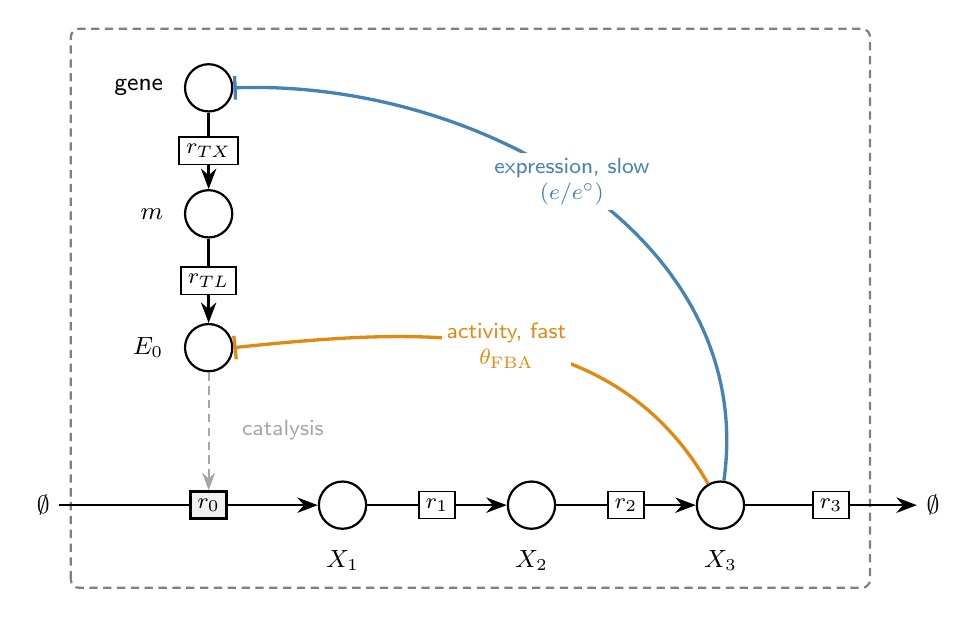
\begin{tikzpicture}[
    font=\small,
    metab/.style   ={circle, draw=black, line width=0.8pt, fill=white,
                     minimum size=6mm, inner sep=0pt},
    rbox/.style    ={draw=black, line width=0.6pt, fill=white, inner sep=2.6pt,
                     font=\footnotesize},
    rboxhi/.style  ={rbox, line width=1.1pt, fill=gray!12},
    flux/.style    ={-{Stealth[length=2.6mm]}, line width=0.9pt},
    cat/.style     ={-{Stealth[length=2.2mm]}, line width=0.8pt, gray!70,
                     densely dashed},
    repress/.style ={-{Bar[width=3mm]}, line width=1.2pt},
  ]

  % ---- system boundary ----
  \begin{scope}[on background layer]
    \draw[densely dashed, gray, line width=0.8pt, rounded corners=3pt]
      (-1.45,-1.05) rectangle (8.7,6.05);
  \end{scope}

  % ---- nodes: metabolic chain (bottom) ----
  \node[metab] (X1) at (2.0,0) {};
  \node[metab] (X2) at (4.4,0) {};
  \node[metab] (X3) at (6.8,0) {};
  \node[below=1.4mm of X1] {$X_1$};
  \node[below=1.4mm of X2] {$X_2$};
  \node[below=1.4mm of X3] {$X_3$};

  % medium (outside the boundary)
  \node (medL) at (-1.8,0) {$\emptyset$};
  \node (medR) at (9.5,0)  {$\emptyset$};

  % ---- nodes: expression cascade (left column) ----
  \node[metab] (E0)   at (0.3,2.0) {};
  \node[metab] (mrna) at (0.3,3.7) {};
  \node[metab] (gene) at (0.3,5.3) {};
  \node[left=1.4mm of E0]   {$E_0$};
  \node[left=1.4mm of mrna] {$m$};
  \node[left=1.4mm of gene] {gene};

  % ---- metabolic flux arrows with reaction boxes ----
  \draw[flux] (medL) -- (X1);
  \node[rboxhi] (rzero) at (0.3,0) {$r_0$};   % placed exactly under E0 (x=0.3)
  \draw[flux] (X1)   -- node[rbox] {$r_1$} (X2);
  \draw[flux] (X2)   -- node[rbox] {$r_2$} (X3);
  \draw[flux] (X3)   -- node[rbox] {$r_3$} (medR);

  % ---- expression flux arrows ----
  \draw[flux] (gene) -- node[rbox] {$r_{TX}$} (mrna);
  \draw[flux] (mrna) -- node[rbox] {$r_{TL}$} (E0);

  % ---- catalysis: E0 enables r0 (straight, E0 sits above r0) ----
  \draw[cat] (E0.south) -- (rzero.north);
  \node[gray!70, font=\footnotesize, anchor=west] at (0.6,0.95) {catalysis};

  % ---- feedback: X3 represses, two loops; each label sits in a white box ON
  %      its own arc (urea EC-box convention) so no line crosses the text ----
  % activity (fast): X3 -| E0
  \draw[repress, actorange] (X3) to[out=120,in=6]
    node[pos=0.5, fill=white, text=actorange, inner sep=1.8pt,
         font=\footnotesize, align=center] {activity, fast\\$\theta_{\mathrm{FBA}}$}
    (E0.east);
  % expression (slow): X3 -| gene
  \draw[repress, exprblue] (X3) to[out=82,in=2]
    node[pos=0.52, fill=white, text=exprblue, inner sep=1.8pt,
         font=\footnotesize, align=center] {expression, slow\\$(e/e^{\circ})$}
    (gene.east);

\end{tikzpicture}
\end{document}
